\documentclass[conference,9pt]{IEEEtran}
\IEEEoverridecommandlockouts
% The preceding line is only needed to identify funding in the first footnote. If that is unneeded, please comment it out.
\usepackage{cite}
\usepackage{amsmath,amssymb,amsfonts,mathtools}
\usepackage{algorithmic}
\usepackage{graphicx}
\usepackage{textcomp}
\usepackage{pdfpages}
\usepackage{multicol}
\usepackage{adjustbox}
\usepackage{multirow}
\usepackage{lipsum}% http://ctan.org/pkg/lipsum
\def\BibTeX{{\rm B\kern-.05em{\sc i\kern-.025em b}\kern-.08em
    T\kern-.1667em\lower.7ex\hbox{E}\kern-.125emX}}
\begin{document}

\title{Energy and Performance Efficient Computation Offloading for Deep Neural Networks in a Mobile Cloud Computing Environment \\
%{\footnotesize \textsuperscript{*}Note: Sub-titles are not captured in Xplore and
%should not be used}
%\thanks{Identify applicable funding agency here. If none, delete this.}
}


\author{
\IEEEauthorblockN{Amir Erfan Eshratifar}
\IEEEauthorblockA{\textit{Department of Electrical Engineering} \\
\textit{University of Southern California}\\
eshratif@usc.edu}
\and
\IEEEauthorblockN{Massoud Pedram}
\IEEEauthorblockA{\textit{Department of Electrical Engineering} \\
\textit{University of Southern California}\\
pedram@usc.edu}
\and
}

\maketitle

\begin{abstract}
In today's computing technology scene, mobile devices are considered to be computationally weak, while large cloud servers are capable of handling expensive workloads, therefore, intensive computing tasks are typically offloaded to the cloud. Recent advances in learning techniques have enabled Deep Neural Networks (DNNs) to be deployed in a wide range of applications. Commercial speech based intelligent personal assistants (IPA) like Apple's Siri, which employs DNN as its recognition model, operate solely over the cloud. The cloud-only approach may require a large amount of data transfer between the cloud and the mobile device. The mobile-only approach may lack performance efficiency. In addition, the cloud server may be slow at times due to the congestion and limited subscription and mobile devices may have battery usage constraints. In this paper, we investigate the efficiency of offloading only some parts of the computations in DNNs to the cloud. We have formulated an optimal computation offloading framework for forward propagation in DNNs, which adapts to battery usage constraints on the mobile side and limited available resources on the cloud. Our simulation results show that our framework can achieve 1.42X on average and up to 3.07X speedup in the execution time on the mobile device. In addition, it results in 2.11x on average and up to 4.26X reduction in mobile energy consumption.
\end{abstract}

\begin{IEEEkeywords}
computation offloading, mobile cloud computing, deep neural networks, energy efficient computing, high performance computing
\end{IEEEkeywords}

\section{Introduction}
With the exponential growth of deep learning techniques and digital raw data, a wide range of applications, that were previously intractable, are enjoying scalable and easy-to-train models. Deep learning has shown extremely promising results in Computer Vision\cite{b1}\cite{b2}, Speech Recognition\cite{b3}, and Natural Language Processing \cite{b4}. Even though, DNNs outperform many other machine learning models, they often require a great amount of computational resources. Mobile devices like smartphones and robots are often considered limited in terms of processing resources and energy budget compared to the cloud server, therefore, DNN workloads are often entirely offloaded to the cloud. However, as the computational resources in the mobile devices are becoming more powerful and energy efficient, we could possibly push some parts of the computations toward the mobile edge.
%Mobile Edge Computing \cite{b5}
Basically, there are following methods during neural networks inferences in mobile cloud computing context:
\begin{enumerate}
\item 
Cloud-only approach: In this method, when the user makes a query, all the input data will be uploaded to the cloud server, afterwards the cloud server does the inference and sends the output back to the mobile. The main drawback of this method is the communication overheads of uploading large inputs (e.g., images, audios, videos), which includes latency and energy costs or downloading large outputs in case of generative models, where the output of the network could be a multimedia file (e.g., image in \cite{b9}). The latency and energy costs of several benchmarks over three different wireless networks (Wi-Fi, 3G, LTE) are studied comprehensively in section \eqref{model}. This approach also compromises user's privacy.
\item 
Mobile-only approach: In this method, all the computations are performed locally in either CPU or GPU depending on the available hardware and software architectures. Recently, Apple has unveiled a new machine learning framework API for developers named Core ML, enabling on-device processing\cite{b10}. They have also included a customized GPU specialized for machine learning tasks in their new smartphone\cite{b28}. In addition, by using this approach, no data will leave the device, which provides more privacy for the user.

\item 
Mobile-cloud collaborative approach: In this method, we seek to develop an optimal scheduling algorithm for collaboratively computation of feed forward neural networks. We break down the computations at layer granularity and decide upon which layers should be computed on mobile and which on the cloud server to achieve maximum performance and energy efficiency. Prior arts in this area often require to transfer the whole process state, which could have potentially large amount of variables to be offloaded, that is not taken into account\cite{b31}. Some rule-based offloading frameworks offload a function, when it is exceeding a pre-defined time ignoring the amount of data to be offloaded\cite{b33}\cite{b32}. In addition, statistical prediction of the execution time and energy of functions used in \cite{b30} are prone to large errors especially in case of DNNs (Section~\ref{profiling}). Our main contribution in this work is formulating optimal computation offloading in DNNs at layer granularity, where the optimality comes from solving an integer linear programming setup.
\end{enumerate}
There are three approaches in estimating the performance and energy consumption of inference with neural networks: 
\begin{itemize}
\item
Statistical modeling by varying the configurable parameters of each layer and measuring the latency and energy consumption for each set of input parameters. A regression model can be used to fit over these profiles so as to estimate the latency and energy of the layer based on its configuration\cite{b29}. In section~\ref{profiling}, we show that the complexities in latency and energy estimation of the conventional layers in deep neural networks are quite high so that it is not feasible to use statistical modeling, because we need exponential number of profiling measurements.
\item
Analytical latency and power modeling by considering hardware and software specifications. State-of-the-art work in latency modeling of deep neural networks \cite{b7} fails to estimate fine-grained layer-level latency within an acceptable error bound. For instance, the delay of 6th layer in VGG-16, which is a fully connected layer with 4096 neurons, is underestimated by around 900 percent. Because of the fact that manufacturers do not reveal the detailed hardware architecture specifications in addition to the proprietary parallel computing architectures like CUDA, analytical approach could be quite challenging\cite{b8}.
\item
Application-specific profiling approach only requires to profile the delay and energy of the target neural networks. Because of the limited number of applications, which requires neural networks in user's mobile, this method seems more practical and leads to more accurate results.
\end{itemize}
In summary, the main contribution of this work is providing a framework to query DNNs efficiently on mobile devices collaborating with cloud server in the presence of battery usage constraints and cloud server limited resources.

\section{Execution time and energy profiling}\label{profiling}

%The only prior study, which investigates a method for task-offloading in deep neural %networks \cite{b2}, only finds one partitioning layer, where all the computations behind %it will be performed on the mobile edge and the rest on the cloud server. 
%This approach will be proved to be not optimal and limited in situations where the cloud %or mobile or both are congested and have constraints on the required energy and %computation capacity.
In this section we elaborate upon the challenges in execution time and energy profiling.
%In addition \cite{b2} turns out to have another major issue in their fine-grained layer-wise delay and energy estimation method, which are far from realistic values. In their work, linear and logarithmic regression methods are established to predict the delay and energy of each layer. As a counter-example to prove that linear and logarithmic regressions are not accurate enough for representing the non-linearity behind the convolution's execution time, we performed four sets of experiments on our mobile platform using Tensorflow\texttrademark 1.0.1\cite{b11} with the following inputs size:
We performed four sets of experiments with the convolution operator, which is generally the most expensive operator in neural networks, on our mobile platform using Tensorflow\texttrademark 1.0.1\cite{b11}. The convolution takes a batch of images of width $img\_w$, height $img\_h$, and with $img\_c$ input channels. The image is convolved with a filter of width $f\_w$, height $f\_h$, and $f\_c$ output channels with a pre-defined stride in $x$ and $y$ directions. The input sizes in our experiments are listed in table~\ref{nonlin_inputs}.
\begin{table}[!ht]
\caption{Convolution inputs size} % title of Table
\label{nonlin_inputs} % is used to refer this table in the text
\centering % used for centering table
\begin{tabular}{|c|c|c|c|c|c|c|c|} % centered columns (4 columns)
%\hline %inserts double horizontal lines
\cline{2-8}
\multicolumn{1}{c|}{} & \textbf{batches} & \textbf{img\_w} & \textbf{img\_h} & \textbf{img\_c} & \textbf{f\_w} & \textbf{f\_h} & \textbf{f\_c} \\ [0.5ex] % inserts table
%heading
\hline % inserts single horizontal line
Case1 & 16 & 64 & 64 & Var & 3 & 3 & 256 \\
\hline % inserts single horizontal line
Case2 & 16 & 64 & 64 & Var & 9 & 9 & 256 \\
\hline % inserts single horizontal line
Case3 & 16 & 64 & 64 & 3 & Var & Var & 256 \\
\hline % inserts single horizontal line
Case4 & 16 & 64 & 64 & 128 & Var & Var & 256 \\
\hline %inserts single line
\end{tabular}
\end{table}
As depicted in Figure~\ref{non-linear-conv}, at some points, increasing the input size decreases the execution time, which is caused by the heuristic selection of different convolution algorithms available in cuDNN\cite{b12}. For instance, for small filter sizes, the convolution is calculated using General Matrix Multiplication (GEMM), while for large filter sizes an algorithm which uses Fast Fourier Transform (FFT) is chosen. Another source of non-linearity is when the GPU is under-utilized and increasing the input size would not affect the execution time.
\begin{figure}[ht]
\centerline{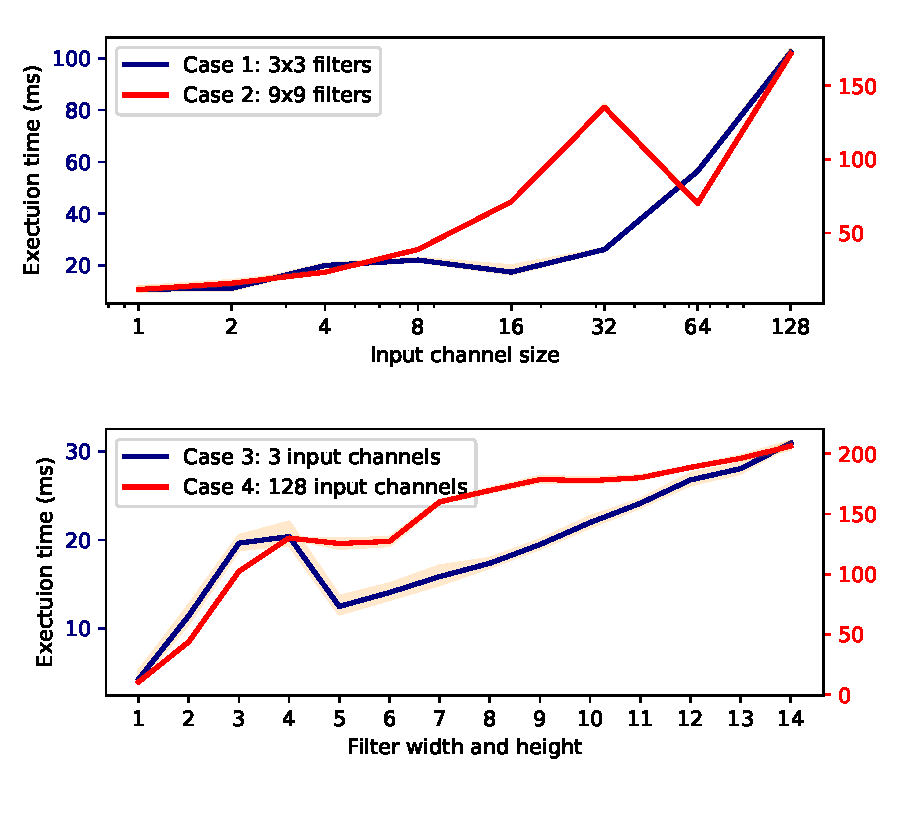
\includegraphics[width=\columnwidth]{convolution_nonlinear_et.pdf}}
\caption{Non-linear execution time of convolutions w.r.t. inputs size. The execution time decreases even when the input size increases because of the heuristic selection of convolution algorithms.}
\label{non-linear-conv}
\end{figure}
Moreover, as depicted in Figure~\ref{consecutive_effect}, layer-wise profiling is prone to large amount of errors in estimation. The reason is the accelerations done by hardware and software frameworks for the consecutive operations. For instance, consider a convolution layer followed by a ReLU\cite{b20}; if an element in the output of the convolution is predicted to be negative at some stage of calculations based on the signs of the inputs, then the rest of the calculations for that element could be discarded, because ReLU will eventually output a zero value. In a nutshell, the execution time of two consecutive layers may not even be close to the sum of the execution times of the individual layers. This fact is depicted in Figure~\ref{consecutive_effect} for AlexNet\cite{b1}. Therefore, for a statistical model we need to profile not only each layer type with different input sizes but also the combination of various layers, which makes the act of profiling and regression very time-consuming and impractical. As a result, we decide to perform application-specific profiling. The level of granularity we are considering in our profiling step, is the following list of the layer types: convolution, deconvolution, pooling, fully connected, and activation functions. 
\begin{figure}[htbp]
\centerline{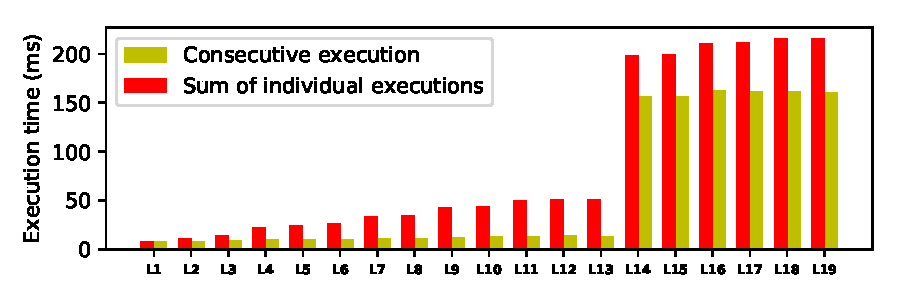
\includegraphics[width=\columnwidth]{consec_effect.pdf}}
\caption{Non-linearity in the execution time of consecutive layers in AlexNet\cite{b1}. Each bar represents the execution time up to that layer.}
\label{consecutive_effect}
\end{figure}
\section{Computation-offloading model for DNN}\label{model}
%Before you begin to format your paper, first write and save the content as a 
%separate text file. Complete all content and organizational editing before 
%formatting. Please note sections \ref{AA}--\ref{SCM} below for more information on 
%proofreading, spelling and grammar.

%Keep your text and graphic files separate until after the text has been 
%formatted and styled. Do not number text heads---{\LaTeX} will do that 
%for you.

%\subsection{Latency and power profiling}\label{AA}
%As mentioned in section
%\begin{itemize}
%\item Use either SI (MKS) or CGS as primary units. (SI units are encouraged.) English units may be used as secondary units (in parentheses). An exception would be the use of English units as identifiers in trade, such as ``3.5-inch disk drive''.
%\item Avoid combining SI and CGS units, such as current in amperes and magnetic field in oersteds. This often leads to confusion because equations do not balance dimensionally. If you must use mixed units, clearly state the units for each quantity that you use in an equation.
%\item Do not mix complete spellings and abbreviations of units: ``Wb/m\textsuperscript{2}'' or ``webers per square meter'', not ``webers/m\textsuperscript{2}''. Spell out units when they appear in text: ``. . . a few henries'', not ``. . . a few H''.
%\item Use a zero before decimal points: ``0.25'', not ``.25''. Use ``cm\textsuperscript{3}'', not ``cc''.)
%\end{itemize}

\subsection{Performance efficient computation offloading setup}
We formulated this problem as an ILP with tractable number of variables. In our method, first we profile the delay and energy consumption of consecutive layers of size $m$ $\in$ $\{1, 2,\dots, num\_layers\}$. We define the number of layers to be $\it{n}$ consistently throughout this paper. Thus, we will have
  \begin{equation}
      \begin{split}
n + (n-1) + ... + 1 = n(n+1)/2
  \end{split}
\end{equation}
number of different profiling values for delay and energy.
Considering i$\it{th}$ layer to j$\it{th}$ layer are computed either on the mobile edge or cloud server, we assign two binary variables $m_{i,j}$ and $c_{i,j}$ respectively. Download and upload communication delays needs to be added to the execution time, while switching to/from cloud from/to mobile respectively.
  \begin{equation}
      \begin{split}
T_{computation} &= \sum_{i=1}^{n}{\sum_{j=i}^{n}{
(m_{i,j}.T_{mobile_{L_{i,j}}} + c_{ij}.T_{cloud_{L_{i,j}}})
}}\label{eq: full_pass_comp}
  \end{split}
\end{equation}
  \begin{equation}
      \begin{split}
T_{communication} &= \sum_{i=1}^{n}{\sum_{j=i}^{n}{\sum_{k=j+1}^{n}{m_{i,j}.c_{j+1,k}.T_{upload_{L_j}}}}} \\
& + \sum_{i=1}^{n}{\sum_{j=i}^{n}{\sum_{k=j+1}^{n}{c_{i,j}.m_{j+1,k}.T_{download_{L_j}}}}} \\
& + \sum_{i=1}^{n}{c_{1,i}.T_{upload_{L_i}}} \\
& + \sum_{i=1}^{n}{c_{i,n}.T_{download_{L_n}}}\label{eq: full_pass_comm}
  \end{split}
\end{equation}
  \begin{equation}
T_{total} = T_{computation} + T_{communication}\thinspace\thinspace\thinspace\thinspace\thinspace\thinspace\thinspace\thinspace\thinspace\thinspace\thinspace\thinspace\thinspace\thinspace\thinspace\thinspace\thinspace\thinspace\thinspace\thinspace\thinspace\thinspace\thinspace\thinspace\thinspace\thinspace\thinspace\thinspace\thinspace\thinspace\thinspace
\end{equation}
$T_{mobile_{L_{i,j}}}$ and $T_{cloud_{L_{i,j}}}$ represent the execution time of $i$th layer to $j$th layer on the mobile and cloud respectively. $T_{download_{L_i}}$ and $T_{upload_{L_i}}$ represent the latency of downloading and uploading the output of $i$th layer respectively. Considering each set of consecutive layers, whenever $m_{i,j}$ and one of $\{c_{j+1,k}\}_{k=j+1:n}$ are one, output of j$\it{th}$ is uploaded to the cloud. The same argument works for download.
We also note that the last two terms in \eqref{eq: full_pass_comm} represent the condition, when last layer is computed on the cloud and we need to download the output to the mobile edge and first layer is computed on the cloud and we need to upload the input to the cloud respectively. Because each set of consecutive layers should be computed either on mobile or cloud or none, we define the following set of constraints:
%$m_{i}$ or $s_{i}$ to be one we define the following constraints:
  \begin{equation}
      \begin{split}
\forall i \in {1:n}, \forall j \in {i:n}:  m_{i,j} + c_{i,j} \leq 1 \label{eq: layers_constraints}
  \end{split}
\end{equation}
Besides, we have to make sure that all layers are being computed exactly once. Therefore, we need to add the following constraints:
  \begin{equation}
      \begin{split}
\forall m \in {1:n}: \sum_{i=1}^{m}{\sum_{j=m}^{n}{(m_{i,j} + c_{i,j})}} = 1
  \end{split}
\end{equation}
Because of the non-linearity of multiplication, an additional step is needed to transform \eqref{eq: full_pass_comm} to the standard form of ILP. We define two sets of new variables: \\
 \begin{equation}\label{eq: download_upload_binary_var} 
 \begin{aligned}
&u_{i,j} = m_{i,j}.\sum_{k=j+1}^{n}{c_{j+1,k}} \\
&d_{i,j} = c_{i,j}.\sum_{k=j+1}^{n}{m_{j+1,k}}
 \end{aligned}\end{equation}
with the following constraints:
\begin{equation}\label{eq: download_upload_constraints} 
 \begin{aligned}
&u_{i,j} \leq m_{i,j}\\
&u_{i,j} \leq \sum_{k=j+1}^{n}{c_{j+1,k}} \\
&m_{i,j} + \sum_{k=j+1}^{n}{c_{j+1,k}} - u_{i,j} \leq 1\\
&d_{i,j} \leq c_{i,j}\\
&d_{i,j} \leq \sum_{k=j+1}^{n}{m_{j+1,k}} \\
&c_{i,j} + \sum_{k=j+1}^{n}{m_{j+1,k}} - d_{i,j} \leq 1
 \end{aligned}
 \end{equation}
 The first two constraints ensure that $u_{i,j}$ will be zero if either $m_{i,j}$ or $\sum_{l=j+1}^{n}{c_{j+1,l}}$ are zero. The third inequality guarantees that $u_{i,j}$ will take value one if both binary variables, $m_{i,j}$ and $\sum_{l=j+1}^{n}{c_{j+1,l}}$, are set to one. The same reasoning works for $d_{i,j}$. In summary, the total number of variables in our ILP formulation will be $4n(n+1)/2$, where $n$ is total number of layers in the network.
\subsection{Energy efficient computation offloading setup}
Because of the nature of the application, we only care about the energy consumption on the mobile side. We formulate ILP as follows:
  \begin{equation}
      \begin{split}
E_{computation} &= \sum_{i=1}^{n}{\sum_{j=i}^{n}{
m_{i,j}.E_{mobile_{L_{i,j}}}}\thinspace\thinspace\thinspace\thinspace\thinspace\thinspace\thinspace\thinspace\thinspace\thinspace\thinspace\thinspace\thinspace\thinspace\thinspace\thinspace\thinspace\thinspace\thinspace\thinspace\thinspace\thinspace\thinspace\thinspace\thinspace\thinspace\thinspace\thinspace\thinspace\thinspace\thinspace\thinspace\thinspace\thinspace\thinspace\thinspace}\label{eq: energy_comp}
  \end{split}
\end{equation}
  \begin{equation}
      \begin{split}
E_{communication} &= \sum_{i=2}^{n}{\sum_{j=i}^{n}{m_{i,j}.E_{download_{L_i}}}} \\
& + \sum_{i=1}^{n}{\sum_{j=i}^{n-1}{m_{i,j}.E_{upload_{L_j}}}} \\
& + (\sum_{i=1}^{n}{(1-m_{1,i}) - (n-1)).E_{upload_{L_1}}} \\
& + (\sum_{i=1}^{n}{(1-m_{i,n}) - (n-1)).E_{download_{L_n}}}\label{eq: energy_comm}
  \end{split}
\end{equation}
  \begin{equation}
E_{total} = E_{computation} + E_{communication}\thinspace\thinspace\thinspace\thinspace\thinspace\thinspace\thinspace\thinspace\thinspace\thinspace\thinspace\thinspace\thinspace\thinspace\thinspace\thinspace\thinspace\thinspace\thinspace
\end{equation}
$E_{mobile_{L_{i,j}}}$ and $E_{cloud_{L_{i,j}}}$ represent the amount of energy required to compute $i$th layer to $j$th layer on the mobile and cloud respectively. $E_{download_{L_i}}$ and $E_{upload_{L_i}}$ represent the amount of energy required to download and upload the output of $i$th layer respectively.
Likewise for performance efficient ILP constraints, we need to make sure that each layer get executed exactly once:
  \begin{equation}
      \begin{split}
\forall m \in {1:n}: \sum_{i=1}^{m}{\sum_{j=m}^{n}{m_{i,j}}} \leq 1
  \end{split}
\end{equation}
%\subsection{Some Common Mistakes}\label{SCM}
%\begin{itemize}
%\item The word ``data'' is plural, not singular.
%\item The subscript for the permeability of vacuum $\mu_{0}$, and other common scientific constants, is zero with subscript formatting, not a lowercase letter ``o''.
%\item In American English, commas, semicolons, periods, question and exclamation marks are located within quotation marks only when a complete thought or name is cited, such as a title or full quotation. When quotation marks are used, instead of a bold or italic typeface, to highlight a word or phrase, punctuation should appear outside of the quotation marks. A parenthetical phrase or statement at the end of a sentence is punctuated outside of the closing parenthesis (like this). (A parenthetical sentence is punctuated within the parentheses.)
%\item A graph within a graph is an ``inset'', not an ``insert''. The word alternatively is preferred to the word ``alternately'' (unless you really mean something that alternates).
%\item Do not use the word ``essentially'' to mean ``approximately'' or ``effectively''.
%\item In your paper title, if the words ``that uses'' can accurately replace the word ``using'', capitalize the ``u''; if not, keep using lower-cased.
%\item Be aware of the different meanings of the homophones ``affect'' and ``effect'', ``complement'' and ``compliment'', ``discreet'' and ``discrete'', ``principal'' and ``principle''.
%\item Do not confuse ``imply'' and ``infer''.
%\item The prefix ``non'' is not a word; it should be joined to the word it modifies, usually without a hyphen.
%\item There is no period after the ``et'' in the Latin abbreviation ``et al.''.
%\item The abbreviation ``i.e.'' means ``that is'', and the abbreviation ``e.g.'' means ``for example''.
%\end{itemize}
%An excellent style manual for science writers is \cite{b7}.
The ILP problem can be solved for different set of parameters (e.g. different uplink and download speeds), and then the scheduling results can be stored as a look-up table in the mobile device. Moreover because the number of variables in this setup is tractable solving ILP is quick. For instance, solving ILP for AlexNet takes around 0.045 seconds on Intel(R) Core(TM) i7-3770 CPU with MATLAB\textregistered's intlinprog() function using primal simplex algorithm.
\subsection{Scenarios}
\begin{itemize}
\item\textbf{Performance efficient computation:} In this case, all we need to do is to solve the ILP formulation for performance efficient computation offloading.
\item\textbf{Energy efficient computation:} In this case, all we need to do is to solve the ILP formulation for energy efficient computation offloading.
\item\textbf{Battery budget limitation:} In this case, according to the available battery, the operating system can decide to dedicate a specific amount of energy usage to each application. By adding the following constraint to the performance efficient ILP formulation, our framework would adapt to battery limitations: 
\begin{equation}
      \begin{split}
E_{computation} + E_{communication} \leq E_{ubound}
  \end{split}
\end{equation}
\item\textbf{Cloud limited resources:} There are situations in which the cloud server is busy or the subscription of the user is limited so that a limit of execution time could be applied to each application to alleviate the server load:
\begin{equation}
      \begin{split}
\sum_{i=1}^{n}{\sum_{j=i}^{n}{
c_{i,j}.T_{cloud_{L_{i,j}}}}} \leq T_{ubound}
  \end{split}
\end{equation}
\end{itemize}
This constraint could be applied to both energy and performance efficient ILP formulations.


%\subsection{Identify the Headings}

%\subsection{Figures and Tables}
%\paragraph{Positioning Figures and Tables}
\section{Case studies}\label{case_studies}
\subsection{Experimental setup}
We use Jetson TX2 board developed by NVIDIA\cite{b18}, which fairly represents the computing power of mobile devices. Our server platform is equipped with NVIDIA\textregistered  Tesla \texttrademark  K40C\cite{b17}, which has 11.25x more computing resources than our mobile platform. We measure the GPU power on our mobile platform using INA226 power monitoring sensor with sampling rate of 500kHz\cite{b21}. In our experiment, we use Tensorflow\texttrademark\cite{b11}, which is an open source software library equipped with cuDNN\cite{b12}, a GPU-accelerated library of primitives for deep neural networks.
Average download and upload speed of mobile networks in the U.S. are considered in this experiment\cite{b13}\cite{b14}. We also use the power models of \cite{b16} for mobile networks with error less than 6\%. The power level for uplink is $P_u = \alpha_u t_u + \beta$ and for downlink is $P_d = \alpha_d t_d + \beta$, where $t_u$ and $t_d$ are uplink and downlink throughputs respectively. The values for our power model paramters are as the following table:
\begin{table}[ht]
\caption{Power model parameters} % title of Table
\centering % used for centering table
\begin{tabular}{|c|c|c|c|} % centered columns (4 columns)
\hline %inserts double horizontal lines
\textbf{Network}& \textbf{$\alpha_u$ (mW/Mpbs)}&\textbf{$\alpha_d$ (mW/Mpbs)}& \textbf{$\beta$ (mW)}\\ [0.5ex] % inserts table
%heading
\hline % inserts single horizontal line
3G & 868.98 & 122.12 & 817.88\\
\hline
4G & 438.39 & 51.97 & 1288.04\\
\hline
Wi-Fi & 283.17 & 137.01 & 132.86\\
\hline %inserts single line
\end{tabular}
\label{table:power_model_parameters} % is used to refer this table in the text
\end{table}
\begin{table}[ht]
\caption{Average download and upload speed of mobile networks in U.S.} % title of Table
\centering % used for centering table
\begin{tabular}{|c|c|c|} % centered columns (4 columns)
\hline %inserts double horizontal lines
\textbf{Network}& \textbf{Download speed (Mpbs)}&\textbf{Upload speed (Mbps)} \\ [0.5ex] % inserts table
%heading
\hline % inserts single horizontal line
3G & 2.0275 & 1.1\\
\hline
4G & 13.76 & 5.85\\
\hline
Wi-Fi & 54.97 & 18.88\\
\hline %inserts single line
\end{tabular}
\label{table:network_speed} % is used to refer this table in the text
\end{table}
\vspace*{-0.2cm}
\begin{table}[ht]
\caption{Mobile device specifications} % title of Table
\centering % used for centering table
\begin{tabular}{|c|c|} % centered columns (4 columns)
\hline %inserts double horizontal lines
\textbf{Component}& \textbf{Specification} \\ [0.5ex] % inserts table
%heading
\hline % inserts single horizontal line
System & Nvidia Jetson TX2 Developer Kit \\
\hline
GPU & NVIDIA Pascal\textregistered, 256 CUDA cores \\
\hline
CPU & HMP Dual Denver + Quad ARM\textregistered A57/2 MB L2 \\
\hline
Memory & 8 GB 128 bit LPDDR4 59.7 GB/s \\ % [1ex] adds vertical space
\hline %inserts single line
\end{tabular}
\label{table:mobile_platform} % is used to refer this table in the text
\end{table}
\vspace*{-0.2cm}
\begin{table}[ht]
\caption{Server platform specifications} % title of Table
\centering % used for centering table
\begin{tabular}{|c|c|} % centered columns (4 columns)
\hline %inserts double horizontal lines
\textbf{Component}& \textbf{Specification} \\ [0.5ex] % inserts table
%heading
\hline % inserts single horizontal line
%System &  \\
%\hline
GPU & NVIDIA \textregistered Tesla\texttrademark K40C, 12GB GDDR5\\
\hline
CPU & Intel \textregistered Xeon \textregistered CPU E7- 8837  @ 2.67GHz \\
\hline
Memory & 64 GB DDR3\\ % [1ex] adds vertical space
\hline %inserts single line
\end{tabular}
\label{table:server_platform} % is used to refer this table in the text
\end{table}

\begin{figure}[htbp]
\centerline{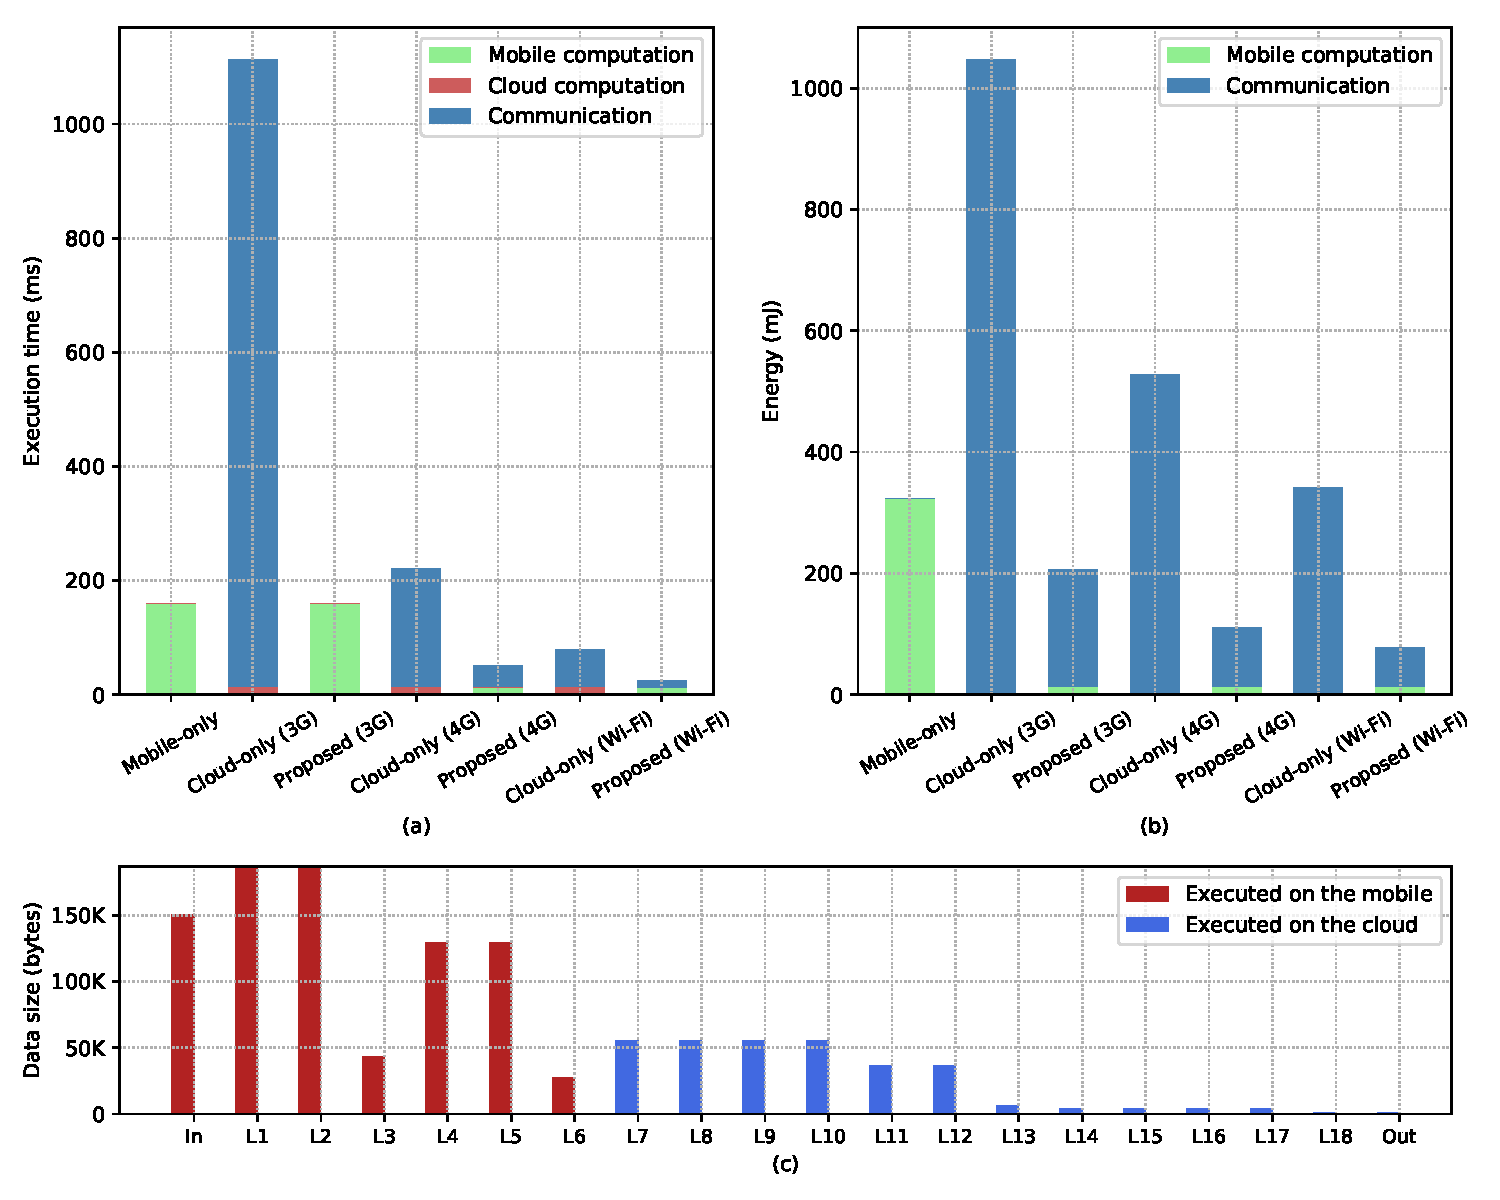
\includegraphics[width=\columnwidth]{alexnet_extracted.pdf}}
\caption{Execution time of AlexNet optimized for performance (a) Mobile energy consumption of AlexNet optimized for energy (b) Data size of the layers in AlexNet and the scheduled computation, where the first seven layers are being computed on the mobile and the rest on the cloud, which is optimal w.r.t. both performance and energy (c).}
\label{alexnet_extracted}
\end{figure}
\begin{figure*}[htbp]
\centerline{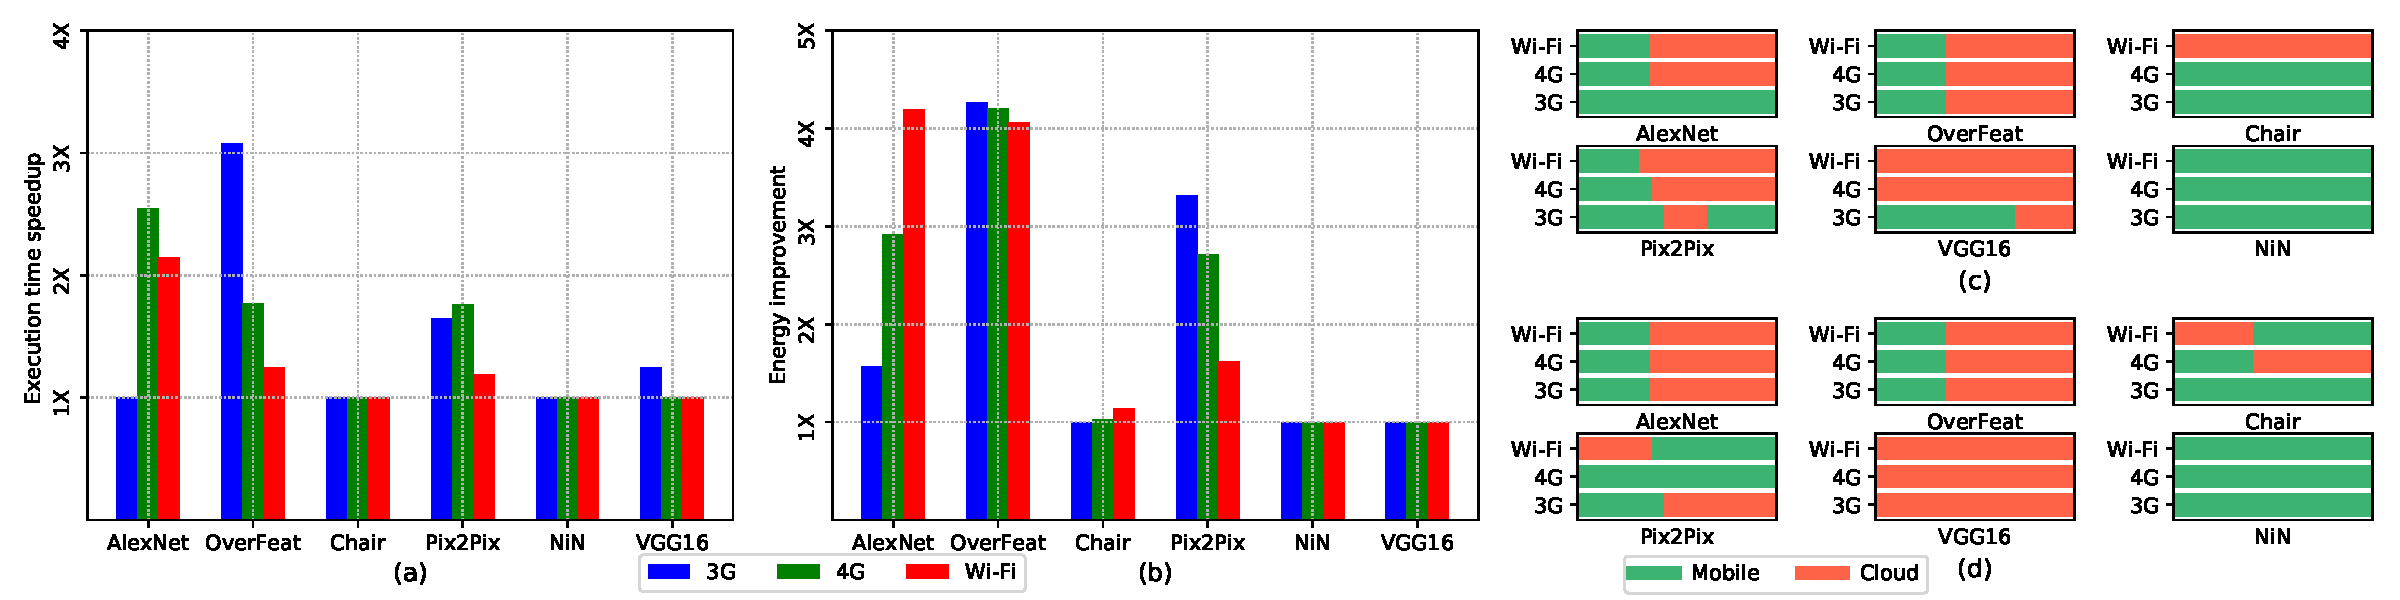
\includegraphics[width=\textwidth]{benchmarks_perf_energy.pdf}}
\caption{Execution time speed up (a) and energy improvement (b) using our proposed framework over the best case of mobile-only and cloud-only approaches. Scheduling patterns in performance efficient (c) and energy efficient (d) setups.}
\label{benchmark_perf_energy}
\end{figure*}
\subsection{Benchmarks}
Since the architecture of neural networks depends on the type of the application, we have chosen three common applications of DNNs:
\begin{enumerate}
\item Discriminative neural networks are a class of models in machine learning for modeling the conditional probability distribution $P(y|x)$. This essentially is used in classification and regression tasks. AlexNet\cite{b1}, OverFeat\cite{b23}, VGG16\cite{b24} and NiN\cite{b22} are the discriminative models we use as benchmarks in this experiment.
\item Generative neural networks model the joint probability distribtion $P(x,y)$, which allows for generating new samples. They have applications in computer vision\cite{b19} and robotics \cite{b15}, which can be deployed on a mobile device. Chair\cite{b25} is a generative model we use as benchmark.
\item Autoencoders are a class of neural networks, which are used to learn a representation for a data set. Their application is in image reconstruction,  image to image translation, and denoising to name a few. Mobile robots can be equipped with autoencoders for their computer vision tasks. We use Pix2Pix\cite{b25}, which has a similar architecture to autoencoders, as our benchmark.
\end{enumerate}

\begin{table}[h]
    \caption{Benchmark Specifications}
\centering
     \begin{adjustbox}{center}
     %\begin{adjustbox}{center}
        \begin{tabular}{|c|c|c|}
        \hline
        \textbf Type & \textbf Model & \textbf Layers \\                
            \hline
            \multirow{4}{*}{Discriminative} & \multicolumn{1}{c}{AlexNet} & \multicolumn{1}{|c|}{19} \\\cline{2-3}
                                 & \multicolumn{1}{c}{OverFeat} & \multicolumn{1}{|c|}{14} \\\cline{2-3}
                                 & \multicolumn{1}{c}{VGG16} & \multicolumn{1}{|c|}{37} \\\cline{2-3}
                                 & \multicolumn{1}{c}{NiN} & \multicolumn{1}{|c|}{29} \\\hline
           Generative & Chair & 10 \\                \hline
            Autoencoder &  Pix2Pix & 32 \\                \hline
        \end{tabular}
     \end{adjustbox}
%     \vspace{ - 05 mm}

    \label{benchmarks}
\end{table}
\subsection{Proposed framework results}
Execution time and energy breakdown for AlexNet, which is noted as a representative for the state-of-the-art models deployed in cloud servers\cite{b27}, is depicted in Figure~\ref{alexnet_extracted}. The cloud-only approach is dominated by the communication costs. As demonstrated in Figure~\ref{alexnet_extracted}, 99\%, 93\% and 81\% of the total execution time is used for communication in case of 3G, 4G, and Wi-Fi. This relative portion also applies to energy consumption. Comparing the latency and energy of the communication to those of mobile-only approach, we figure out that mobile-only approach for AlexNet is better than the cloud-only approach in all the mobile networks.\\

Figure~\ref{benchmark_perf_energy} shows the execution time and energy improvements for 6 different benchmarks. We have considered the best case of cloud-only and mobile-only as our baseline. We have also depicted the schedule of computations in this figure. As we can see, the cloud-only and mobile-only approaches are optimal for VGG16 and NiN respectively, while optimizing for mobile energy consumption. Our proposed framework can achieve 1.42X on average and up to 3.07X (OverFeat, 3G) speedup when optimizing for performance. Mobile energy consumption can be reduced 2.11X on average and up to 4.26X (OverFeat, 3G), while optimizing for energy consumption. The improvements in the execution time of deep neural networks benefits not only the mobile users but also the cloud providers, which essentially means that they could save more resources or have more users. Another key observation is the scheduling pattern of the computations in different types of neural networks. Generally, in discriminative networks, the input size is often large and the output size is small, which implies that it is better to compute the first layers on the mobile to avoid uploading large inputs to the cloud. On the other hand, in generative networks, output size is often large, which implies that it is better to compute the last layers on the mobile to avoid downloading large outputs from the cloud. In autoencoders, both the input and output data sizes are often large, therefore, it is better to compute the first and last layers on the mobile and offload the computations in the middle layers to the cloud.

\subsection{Cloud limited available resources experiment}
The cloud resource management may decide to allow a process to be executed for a limited amount of time. The reason could be the user's limited subscription or congestion in the cloud server. In this scenario, we have set up a experiment in which the cloud allows up to 50\% of the execution time of the whole neural network on the cloud over Wi-Fi network setup. As we have shown in the Figure ~\ref{constraints_effect}, multiple data transfer points may occur, whose maximum is four in case of OverFeat.
\begin{figure}[htbp]
\centerline{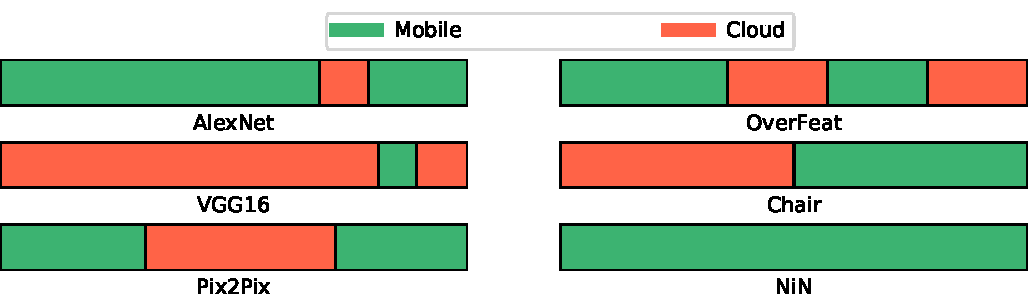
\includegraphics[width=\columnwidth]{constraints_effect.pdf}}
\caption{Computation scheduling patterns under execution time constraint of the cloud over Wi-Fi network setup}
\label{constraints_effect}
\end{figure}
\section*{Conclusion and Roadmap}
In this work, we demonstrated that cloud-only or mobile-only approaches are not necessarily optimal with regard to performance and energy. We formulated the problem with ILP setup, which is solved only once by the cloud server. The reason that we are using ILP is the fact that the number of data transfer points strongly depends on the network architecture and resource constraints applied by the cloud and mobile. It is possible to limit the number of data transfer points and solve the problem by a polynomial algorithm, but it is not guaranteed to be optimal for all kinds of network architecture and constraints.
The output data size of generative models, are generally large so the last layers are expected to be computed on the mobile in the optimal case to avoid downloading large data. On the other hand, classification networks have smaller output data size, therefore last layers are expected to be computed on the cloud. Autoencoders have large input and output data sizes, which implies that the first and last layers are expected to be computed on the mobile. With these insights, the computation scheduling of deep neural networks can possibly have different patterns depending on the model architecture. The proposed framework in this paper can be extended to any data flow computational graphs with the granularity of primitive operators like multiplication.
\section*{Acknowledgment}
This research was supported by grants from NSF SHF and DARPA MTO. 
\begin{thebibliography}{00}
\bibitem{b1} Krizhevsky et al., Imagenet classification with deep convolutional
neural networks, NIPS, 2012.
\bibitem{b2} Karen Simonyan and Andrew Zisserman. Very deep convolutional
networks for large-scale image recognition. preprint arXiv:1409.1556, 2014.
\bibitem{b3} Hinton, G. et al. Deep neural networks for acoustic modeling in speech recognition. IEEE Signal Processing Magazine 29, 2012.
\bibitem{b4} Collobert, R., et al. Natural language processing (almost) from scratch. J. Mach. Learn. Res. 12, 2493–2537, 2011.
\bibitem{b7} Hang Qi, Evan R. Sparks, and Ameet Talwalkar. Paleo: A Performance Model for Deep Neural Networks. International Conference on Learning Representations, 2017.
\bibitem{b8} Sunpyo Hong and Hyesoon Kim. An integrated GPU power and performance model. In Proceedings of the 37th annual international symposium on Computer architecture, 2010.
\bibitem{b9} Alec Radford, Luke Metz, Soumith Chintala:
Unsupervised Representation Learning with Deep Convolutional Generative Adversarial Networks. CoRR abs/1511.06434, 2015.
\bibitem{b10} Apple announces new machine learning API to make mobile AI faster https://www.theverge.com/2017/6/5/15725994/apple-mobile-ai-chip-announced-wwdc-2017
\bibitem{b11}M. Abadi, A. Agarwal et al., Tensorflow: Large-scale
machine learning on heterogeneous distributed systems, arXiv:1603.04467, 2016.
\bibitem{b12} NVIDIA cuDNN https://developer.nvidia.com/cudnn
\bibitem{b13} State of Mobile Networks: USA - OpenSignal https://opensignal.com/reports/2017/08/usa/state-of-the-mobile-network
\bibitem{b14} 2017 United States Speedtest Market Report http://www.speedtest.net/reports/united-states/
\bibitem{b15} Finn, C. and Levine, S. Deep visual foresight for planning robot motion. arXiv preprint arXiv:1610.00696, 2016.
\bibitem{b16} Junxian Huang, Feng Qian, Alexandre Gerber, Z. Morley Mao, Subhabrata Sen, and Oliver Spatscheck. A close examination of performance and power characteristics of 4G LTE networks. In Proceedings of the 10th international conference on Mobile systems, applications, and services, 2012.
\bibitem{b17} Tesla GPU Accelerators for Servershttp://www.nvidia.com/object/tesla-servers.html
\bibitem{b18} Jetson TX2 Module https://developer.nvidia.com/embedded/buy/jetson-tx2
\bibitem{b19} Ian J. Goodfellow, Jean Pouget-Abadie et al., “Generative Adversarial Networks,” arXiv:1406.2661, 2014.
\bibitem{b20} Vinod Nair and Geoffrey E. Hinton. Rectified linear units improve restricted boltzmann machines. In Proceedings of the 27th International Conference on International Conference on Machine Learning, 2010.
\bibitem{b21} INA226 http://www.ti.com/product/INA226
\bibitem{b22} Min Lin, Qiang Chen, Shuicheng Yan, Network In Network. arXiv preprint arXiv:1312.4400, 2014.
\bibitem{b23} Pierre Sermanet et al., OverFeat: Integrated Recognition, Localization and Detection using Convolutional Networks. arXiv:1312.6229, 2014.
\bibitem{b24} Karen Simonyan, Andrew Zisserman, Very Deep Convolutional Networks for Large-Scale Image Recognition. arXiv:1409.1556, 2014.
\bibitem{b25} Alexey Dosovitskiy et al., Learning to Generate Chairs, Tables and Cars with Convolutional Networks. arXiv:1411.5928, 2017.
\bibitem{b26} Phillip Isola, Jun-Yan Zhu, Tinghui Zhou, Alexei A. Efros, Image-to-Image Translation with Conditional Adversarial Networks. arXiv:1611.07004, 2016.
\bibitem{b27} Adam Coates, Brody Huval, Tao Wang, David J. Wu, Andrew Y. Ng, and Bryan Catanzaro. Deep learning with COTS HPC systems. In Proceedings of the 30th International Conference on International Conference on Machine Learning, 2013.
\bibitem{b28} The new iPhone 8 has a custom GPU designed by Apple with its new A11 Bionic chip https://techcrunch.com/2017/09/12/the-new-iphone-8-has-a-custom-gpu-designed-by-apple-with-its-new-a11-bionic-chip/
\bibitem{b29} Yiping Kang, Johann Hauswald, Cao Gao, Austin Rovinski, Trevor Mudge, Jason Mars, and Lingjia Tang. Neurosurgeon: Collaborative Intelligence Between the Cloud and Mobile Edge. SIGARCH Comput. Archit, 2017.
\bibitem{b30} Eduardo Cuervo et al., Maui: making smartphones last longer with code offload. In Proceedings of the 8th international conference on Mobile systems, applications, and services, ACM, 2010.
\bibitem{b31} Roelof KempNicholas PalmerThilo KielmannHenri Bal, Cuckoo: A Computation Offloading Framework for Smartphones, International Conference on Mobile Computing, Applications, and Services, 2010.
\bibitem{b32} Mark S Gordon, Davoud Anoushe Jamshidi, Scott A Mahlke, Zhuoqing Morley Mao, and Xu Chen. Comet: Code offload
by migrating execution transparently, 2012.
\bibitem{b33} Byung-Gon Chun, Sunghwan Ihm, Petros Maniatis, Mayur Naik, and Ashwin Patti. CloneCloud: elastic execution between mobile device and cloud. In Proceedings of the sixth conference on Computer systems, 2011.
\end{thebibliography}

\end{document}
